\documentclass[11pt, twocolumn]{article}

\usepackage{graphics}
\usepackage{hyperref}
\usepackage[usenames, dvipsnames]{color}
\usepackage{colortbl}

% Sans fonts
\usepackage{sfmath}
\renewcommand{\familydefault}{\sfdefault}

\newcommand{\COURSE}{PHYS328W}
\newcommand{\TITLE}{Reference}
\markright{\COURSE\ : \TITLE}

\setlength{\textwidth} {6.5 true in}
\setlength{\textheight}{9 true in}
%\setlength{\hoffset}   {-0.50 true in}
\setlength{\voffset}   {-0.75 true in}
\setlength{\parindent} {12 pt}
\pagestyle{myheadings}
\pagenumbering{gobble}

\begin{document}

\subsubsection*{Ohmic Devices}
\begin{center}
$V = IR$\\
$P_\mathrm{diss} = I^2 R = \frac{V^2}{R}$
\end{center}

\subsubsection*{Resistors in Series and Parallel}
\begin{center}
\scalebox{0.75}{
  \includegraphics{seriesparallel.eps}
}

{\renewcommand{\arraystretch}{1.5}
\begin{tabular}{rl}
\textbf{Series:}   & $R_{eq} = R_1 + R_2 + R_3 + \ldots$\\
                   & $V_1 = \frac{R_1}{R_1 + R_2} V$\\
\textbf{Parallel:} & $\frac{1}{R_{eq}} = \frac{1}{R_1} + \frac{1}{R_2} + \frac{1}{R_3} + \ldots$\\
                   & $\Delta I_1 = \frac{R_2}{R_1 + R_2} I$ 
\end{tabular}
}
\end{center}

\subsubsection*{Kirchhoff's Rules}
\begin{center}
{\renewcommand{\arraystretch}{1.5}
\begin{tabular}{rl}
\textbf{Loop Rule:}     & $\sum_\mathrm{loop} V_i = 0$\\
\textbf{Junction Rule:} & $\sum_\mathrm{junction} I_i = 0$
\end{tabular}
}
\end{center}

\subsubsection*{Phasor Analysis}
\begin{center}
$X_L = j \omega L$ \hspace{3 cm} $X_C = -\frac{j}{\omega C}$\\
$\mathbf{V} = V \, e^{\,j \phi_v}$ \hspace{3 cm}
$\mathbf{I} = I \, e^{\,j \phi_i}$\\
$\mathbf{I} = \frac{\mathbf{V}}{Z}$\\
$v(t) = Re(\mathbf{V} \, e^{\,j\omega t})$ \hspace{1.5 cm}
$i(t) = Re(\mathbf{I} \, e^{\,j\omega t})$\\
$\left< P \right> = \frac{IV}{2} \cos(\phi_v - \phi_i)
                 = \frac{V^2}{2Z} \cos(\phi_v - \phi_i)$
\end{center}
\textbf{AC Voltage Divider}
\begin{center}
$\frac{V_{out}}{V_{in}} = \frac{|\mathbf{V_{out}}|}{|\mathbf{V_{in}}|}
  = \left| \frac{Z_2}{Z_1 + Z_2} \right|
  = \sqrt{ \left( \frac{Z_2}{Z_1 + Z_2} \right)^*
           \left( \frac{Z_2}{Z_1 + Z_2} \right) }$\\
$\tan \phi = \frac{ Im \left( \frac{Z_2}{Z_1 + Z_2} \right) }
                { Re \left( \frac{Z_2}{Z_1 + Z_2} \right) }$
\end{center}

\subsubsection*{Resistor Color Codes}

\begin{center}
\begin{tabular}{|r|r|r|}\hline
\textbf{color} & \textbf{digit} & \textbf{multiplier} \\\hline
\color{white}\cellcolor{Black}black & 0 & 1     \\\hline
\color{white}\cellcolor{Brown}brown & 1 & 10    \\\hline
\cellcolor{Red}red                  & 2 & 100   \\\hline
\cellcolor{Orange}orange            & 3 & 1k    \\\hline
\cellcolor{Yellow}yellow            & 4 & 10k   \\\hline
\cellcolor{Green}green              & 5 & 100k  \\\hline
\cellcolor{Blue}blue                & 6 & 1M    \\\hline
\cellcolor{Purple}violet            & 7 & 10M   \\\hline
\cellcolor{Gray}gray                & 8 & 100M  \\\hline
white                               & 9 & 1000M \\\hline
\end{tabular}
\begin{eqnarray*}
R = [\mathrm{band 1}][\mathrm{band 2}] 
    \times 10^{[\mathrm{band 3}]} & \pm & 5\%~(\mathrm{gold})\\ 
                                  & \pm & 10\%~(\mathrm{silver})\nonumber
\end{eqnarray*}
\end{center}

\subsubsection*{Breadboard Layout}
\begin{center}
  \scalebox{0.4}{
    \includegraphics{breadboard.eps}
  }
\end{center}

\subsubsection*{Schematic Symbols}
\begin{center}
  \scalebox{0.8}{
    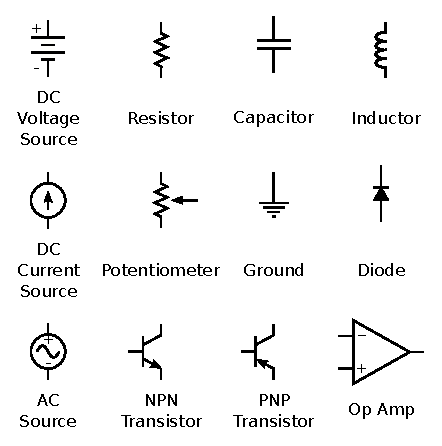
\includegraphics{schematic.eps}
  }
  
  \vspace{24 pt}

  \scalebox{0.5}{
    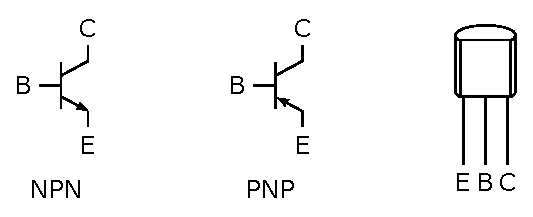
\includegraphics{transistors_ref.eps}
  }
\end{center}

\end{document}
